%% 
%% Copyright 2019-2020 Elsevier Ltd
%% 
%% This file is part of the 'CAS Bundle'.
%% --------------------------------------
%% 
%% It may be distributed under the conditions of the LaTeX Project Public
%% License, either version 1.2 of this license or (at your option) any
%% later version.  The latest version of this license is in
%%    http://www.latex-project.org/lppl.txt
%% and version 1.2 or later is part of all distributions of LaTeX
%% version 1999/12/01 or later.
%% 
%% The list of all files belonging to the 'CAS Bundle' is
%% given in the file `manifest.txt'.
%% 
%% Template article for cas-dc documentclass for 
%% double column output.

%\documentclass[a4paper,fleqn,longmktitle]{cas-dc}
\documentclass[a4paper,fleqn]{cas-dc}

%\usepackage[authoryear,longnamesfirst]{natbib}
%\usepackage[authoryear]{natbib}
\usepackage[numbers]{natbib}

%%%Author definitions
\def\tsc#1{\csdef{#1}{\textsc{\lowercase{#1}}\xspace}}
\tsc{WGM}
\tsc{QE}
\tsc{EP}
\tsc{PMS}
\tsc{BEC}
\tsc{DE}
%%%
% -------------------------------------------------------------------
% Pacotes para inserção de figuras e subfiguras
\usepackage{subfig,epsfig,tikz,float}		            % Packages de figuras. 
\usepackage{graphicx}
\graphicspath{ {./figs/} }
% -------------------------------------------------------------------
% \usepackage{amssymb}
% -------------------------------------------------------------------
% Pacotes para inserção de tabelas
\usepackage{booktabs,multicol,multirow,tabularx,array}          % Packages para tabela
\usepackage{natbib}
\usepackage{pifont}
\usepackage{xcolor}
% -------------------------------------------------------------------
\PassOptionsToPackage{style=super,nolist}{glossaries}
\PassOptionsToPackage{acronym}{glossaries}
\PassOptionsToPackage{nonumberlist}{glossaries}
\usepackage{glossaries}
\newacronym{ai}{AI}{Artificial Intelligence}
\makeglossaries
% -------------------------------------------------------------------
\usepackage[utf8]{inputenc} % The default since 2018
\DeclareUnicodeCharacter{200B}{{\hskip 0pt}}
% -------------------------------------------------------------------
\begin{document}
\let\WriteBookmarks\relax
\def\floatpagepagefraction{1}
\def\textpagefraction{.001}
\shorttitle{Leveraging social media news}
\shortauthors{CV Radhakrishnan et~al.}

\title [mode = title]{This is a specimen $a_b$ title}                      
\tnotemark[1,2]

\tnotetext[1]{This document is the results of the research
   project funded by the National Science Foundation.}

\tnotetext[2]{The second title footnote which is a longer text matter
   to fill through the whole text width and overflow into
   another line in the footnotes area of the first page.}



\author[1,3]{CV Radhakrishnan}[type=editor,
                        auid=000,bioid=1,
                        prefix=Sir,
                        role=Researcher,
                        orcid=0000-0001-7511-2910]
\cormark[1]
\fnmark[1]
\ead{cvr_1@tug.org.in}
\ead[url]{www.cvr.cc, cvr@sayahna.org}

\credit{Conceptualization of this study, Methodology, Software}

\address[1]{Elsevier B.V., Radarweg 29, 1043 NX Amsterdam, The Netherlands}

\author[2,4]{Han Theh Thanh}[style=chinese]

\author[2,3]{CV Rajagopal}[%
   role=Co-ordinator,
   suffix=Jr,
   ]
\fnmark[2]
\ead{cvr3@sayahna.org}
\ead[URL]{www.sayahna.org}

\credit{Data curation, Writing - Original draft preparation}

\address[2]{Sayahna Foundation, Jagathy, Trivandrum 695014, India}

\author%
[1,3]
{Rishi T.}
\cormark[2]
\fnmark[1,3]
\ead{rishi@stmdocs.in}
\ead[URL]{www.stmdocs.in}

\address[3]{STM Document Engineering Pvt Ltd., Mepukada,
    Malayinkil, Trivandrum 695571, India}

\cortext[cor1]{Corresponding author}
\cortext[cor2]{Principal corresponding author}
\fntext[fn1]{This is the first author footnote. but is common to third
  author as well.}
\fntext[fn2]{Another author footnote, this is a very long footnote and
  it should be a really long footnote. But this footnote is not yet
  sufficiently long enough to make two lines of footnote text.}

\nonumnote{This note has no numbers. In this work we demonstrate $a_b$
  the formation Y\_1 of a new type of polariton on the interface
  between a cuprous oxide slab and a polystyrene micro-sphere placed
  on the slab.
  }

\begin{abstract}
This template helps you to create a properly formatted \LaTeX\ manuscript.

\noindent\texttt{\textbackslash begin{abstract}} \dots 
\texttt{\textbackslash end{abstract}} and
\verb+\begin{keyword}+ \verb+...+ \verb+\end{keyword}+ 
which
contain the abstract and keywords respectively. 

\noindent Each keyword shall be separated by a \verb+\sep+ command.
\end{abstract}

\begin{graphicalabstract}
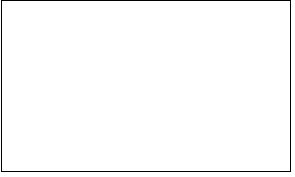
\includegraphics{figs/grabs.pdf}
\end{graphicalabstract}

\begin{highlights}
\item Research highlights item 1
\item Research highlights item 2
\item Research highlights item 3
\end{highlights}

\begin{keywords}
quadrupole exciton \sep polariton \sep \WGM \sep \BEC
\end{keywords}


\maketitle

\section{Introduction}

Abbreviation Example: \gls{ai} \\
Citation Example: \cite{Blondeletal2008}
Text Text Text Text Text Text Text Text Text Text Text Text Text Text Text Text Text Text Text Text Text Text Text Text Text Text Text Text Text Text Text Text Text Text Text Text Text Text Text Text Text Text Text Text Text Text Text Text Text Text Text Text Text Text Text Text Text Text Text Text Text Text Text Text Text Text Text Text Text Text Text Text Text Text Text Text Text Text Text Text Text Text Text Text Text Text Text Text Text Text Text Text Text Text Text Text Text Text Text Text Text Text Text Text Text Text Text Text Text Text Text Text Text Text Text Text Text Text Text Text Text Text Text Text Text Text Text Text Text Text Text Text Text Text Text Text Text Text Text Text Text Text Text Text Text Text Text Text Text Text Text Text 
This class depends on the following packages
for its proper functioning:

\printcredits

%% Loading bibliography style file
%\bibliographystyle{model1-num-names}
%\bibliographystyle{cas-model2-names}
\bibliographystyle{plain} % Estilo de Bibliografia
% Loading bibliography database
\bibliography{cas-refs}


%\vskip3pt

\bio{}
Author biography without author photo.
Author biography. Author biography. Author biography.
Author biography. Author biography. Author biography.
Author biography. Author biography. Author biography.
Author biography. Author biography. Author biography.
Author biography. Author biography. Author biography.
Author biography. Author biography. Author biography.
Author biography. Author biography. Author biography.
Author biography. Author biography. Author biography.
Author biography. Author biography. Author biography.
\endbio

\bio{figs/pic1}
Author biography with author photo.
Author biography. Author biography. Author biography.
Author biography. Author biography. Author biography.
Author biography. Author biography. Author biography.
Author biography. Author biography. Author biography.
Author biography. Author biography. Author biography.
Author biography. Author biography. Author biography.
Author biography. Author biography. Author biography.
Author biography. Author biography. Author biography.
Author biography. Author biography. Author biography.
\endbio

\bio{figs/pic1}
Author biography with author photo.
Author biography. Author biography. Author biography.
Author biography. Author biography. Author biography.
Author biography. Author biography. Author biography.
Author biography. Author biography. Author biography.
\endbio

\end{document}
